Scan-matching is employed in robotics as a means to odometry,
primarily in non-wheeled robots where no encoders can be utilised, or as a
useful ameliorator of the ever-drifting encoder-ed odometry: scans captured at
consecutive time instances, inputted to a scan-matching algorithm, convey an
estimate as to the pose of the scan sensor at the second capture time
relative to that captured first. Scan-matching is being successfully employed
in the tasks of simultaneous localisation and mapping
\cite{am_odom_1}-\cite{am_odom_3}, local map construction
\cite{am_odom_4}-\cite{am_odom_6}, and in people-tracking systems
\cite{am_odom_7}.

cannot stress enough: the contributions must be layed out and emphasised
see. olsen 2009 for a pro

Contribution: invariant to large angular errors, pseudoinvariant in time of execution, show how to decrease orientation error from fixed number of rays, fourier for both orientation and translation --> robustness,
not many panoramic 2d scan matchers out there (are there any?): recent years have seen intro of
cheap panoramic sensors. we exploit properties of fourier for ...

fewer parameters


% Maybe motivate panoramic: new sensors, much noise; robustness? or just in the
% introduction/contribution


\begin{figure}[]\centering
  % GNUPLOT: LaTeX picture with Postscript
\begingroup
  \makeatletter
  \providecommand\color[2][]{%
    \GenericError{(gnuplot) \space\space\space\@spaces}{%
      Package color not loaded in conjunction with
      terminal option `colourtext'%
    }{See the gnuplot documentation for explanation.%
    }{Either use 'blacktext' in gnuplot or load the package
      color.sty in LaTeX.}%
    \renewcommand\color[2][]{}%
  }%
  \providecommand\includegraphics[2][]{%
    \GenericError{(gnuplot) \space\space\space\@spaces}{%
      Package graphicx or graphics not loaded%
    }{See the gnuplot documentation for explanation.%
    }{The gnuplot epslatex terminal needs graphicx.sty or graphics.sty.}%
    \renewcommand\includegraphics[2][]{}%
  }%
  \providecommand\rotatebox[2]{#2}%
  \@ifundefined{ifGPcolor}{%
    \newif\ifGPcolor
    \GPcolorfalse
  }{}%
  \@ifundefined{ifGPblacktext}{%
    \newif\ifGPblacktext
    \GPblacktexttrue
  }{}%
  % define a \g@addto@macro without @ in the name:
  \let\gplgaddtomacro\g@addto@macro
  % define empty templates for all commands taking text:
  \gdef\gplbacktext{}%
  \gdef\gplfronttext{}%
  \makeatother
  \ifGPblacktext
    % no textcolor at all
    \def\colorrgb#1{}%
    \def\colorgray#1{}%
  \else
    % gray or color?
    \ifGPcolor
      \def\colorrgb#1{\color[rgb]{#1}}%
      \def\colorgray#1{\color[gray]{#1}}%
      \expandafter\def\csname LTw\endcsname{\color{white}}%
      \expandafter\def\csname LTb\endcsname{\color{black}}%
      \expandafter\def\csname LTa\endcsname{\color{black}}%
      \expandafter\def\csname LT0\endcsname{\color[rgb]{1,0,0}}%
      \expandafter\def\csname LT1\endcsname{\color[rgb]{0,1,0}}%
      \expandafter\def\csname LT2\endcsname{\color[rgb]{0,0,1}}%
      \expandafter\def\csname LT3\endcsname{\color[rgb]{1,0,1}}%
      \expandafter\def\csname LT4\endcsname{\color[rgb]{0,1,1}}%
      \expandafter\def\csname LT5\endcsname{\color[rgb]{1,1,0}}%
      \expandafter\def\csname LT6\endcsname{\color[rgb]{0,0,0}}%
      \expandafter\def\csname LT7\endcsname{\color[rgb]{1,0.3,0}}%
      \expandafter\def\csname LT8\endcsname{\color[rgb]{0.5,0.5,0.5}}%
    \else
      % gray
      \def\colorrgb#1{\color{black}}%
      \def\colorgray#1{\color[gray]{#1}}%
      \expandafter\def\csname LTw\endcsname{\color{white}}%
      \expandafter\def\csname LTb\endcsname{\color{black}}%
      \expandafter\def\csname LTa\endcsname{\color{black}}%
      \expandafter\def\csname LT0\endcsname{\color{black}}%
      \expandafter\def\csname LT1\endcsname{\color{black}}%
      \expandafter\def\csname LT2\endcsname{\color{black}}%
      \expandafter\def\csname LT3\endcsname{\color{black}}%
      \expandafter\def\csname LT4\endcsname{\color{black}}%
      \expandafter\def\csname LT5\endcsname{\color{black}}%
      \expandafter\def\csname LT6\endcsname{\color{black}}%
      \expandafter\def\csname LT7\endcsname{\color{black}}%
      \expandafter\def\csname LT8\endcsname{\color{black}}%
    \fi
  \fi
    \setlength{\unitlength}{0.0500bp}%
    \ifx\gptboxheight\undefined%
      \newlength{\gptboxheight}%
      \newlength{\gptboxwidth}%
      \newsavebox{\gptboxtext}%
    \fi%
    \setlength{\fboxrule}{0.5pt}%
    \setlength{\fboxsep}{1pt}%
\begin{picture}(5000.00,5000.00)%
    \gplgaddtomacro\gplbacktext{%
      \colorrgb{0.15,0.15,0.15}%
      \put(391,1564){\makebox(0,0)[r]{\strut{}$6.0$}}%
      \colorrgb{0.15,0.15,0.15}%
      \put(391,1988){\makebox(0,0)[r]{\strut{}$8.0$}}%
      \colorrgb{0.15,0.15,0.15}%
      \put(391,2413){\makebox(0,0)[r]{\strut{}$10.0$}}%
      \colorrgb{0.15,0.15,0.15}%
      \put(391,2837){\makebox(0,0)[r]{\strut{}$12.0$}}%
      \colorrgb{0.15,0.15,0.15}%
      \put(391,3262){\makebox(0,0)[r]{\strut{}$14.0$}}%
      \colorrgb{0.15,0.15,0.15}%
      \put(391,3687){\makebox(0,0)[r]{\strut{}$16.0$}}%
      \colorrgb{0.00,0.00,0.00}%
      \put(672,1280){\makebox(0,0){\strut{}$-2.0$}}%
      \colorrgb{0.00,0.00,0.00}%
      \put(1096,1280){\makebox(0,0){\strut{}$0.0$}}%
      \colorrgb{0.00,0.00,0.00}%
      \put(1521,1280){\makebox(0,0){\strut{}$2.0$}}%
      \colorrgb{0.00,0.00,0.00}%
      \put(1945,1280){\makebox(0,0){\strut{}$4.0$}}%
      \colorrgb{0.00,0.00,0.00}%
      \put(2370,1280){\makebox(0,0){\strut{}$6.0$}}%
    }%
    \gplgaddtomacro\gplfronttext{%
    }%
    \gplgaddtomacro\gplbacktext{%
      \colorrgb{0.00,0.00,0.00}%
      \put(2822,1280){\makebox(0,0){\strut{}$-2.0$}}%
      \colorrgb{0.00,0.00,0.00}%
      \put(3246,1280){\makebox(0,0){\strut{}$0.0$}}%
      \colorrgb{0.00,0.00,0.00}%
      \put(3671,1280){\makebox(0,0){\strut{}$2.0$}}%
      \colorrgb{0.00,0.00,0.00}%
      \put(4095,1280){\makebox(0,0){\strut{}$4.0$}}%
      \colorrgb{0.00,0.00,0.00}%
      \put(4520,1280){\makebox(0,0){\strut{}$6.0$}}%
    }%
    \gplgaddtomacro\gplfronttext{%
    }%
    \gplbacktext
    \put(0,0){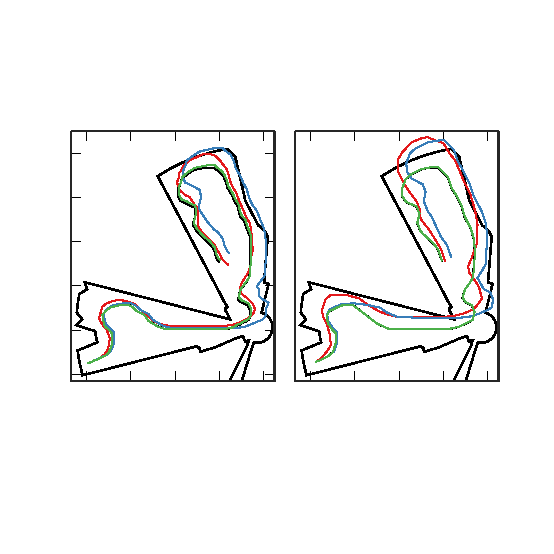
\includegraphics{./figures/odom_test_5_vs_6}}%
    \gplfronttext
  \end{picture}%
\endgroup

  \caption{\small}
  \label{fig:}
\end{figure}

\begin{figure}[]\centering
  

\tikzset{every picture/.style={line width=0.75pt}} %set default line width to 0.75pt

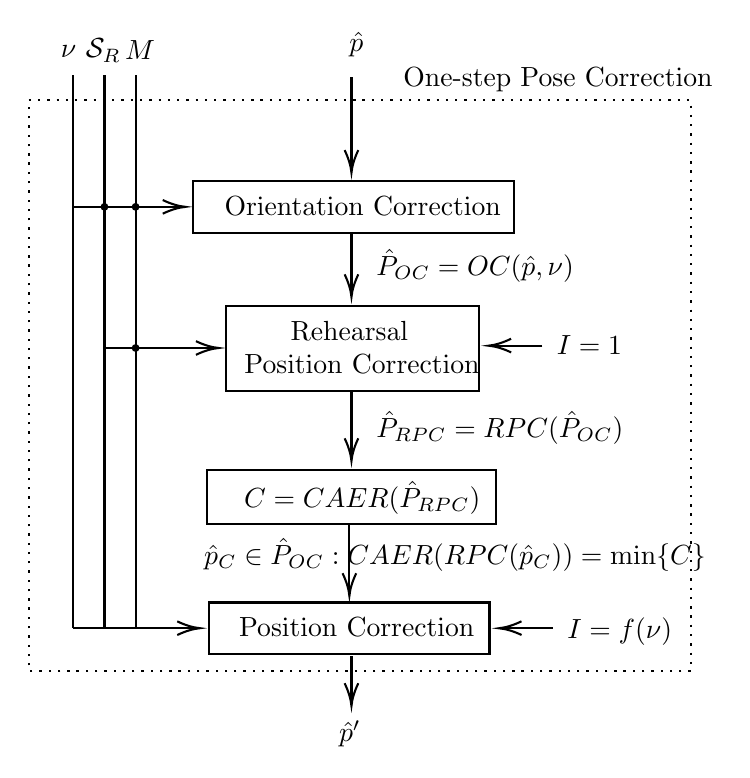
\begin{tikzpicture}[x=0.75pt,y=0.75pt,yscale=-1,xscale=1]
%uncomment if require: \path (0,542); %set diagram left start at 0, and has height of 542

%Straight Lines [id:da5372026622110897]
\draw    (126.5,63) -- (126.5,329.29) ;
%Straight Lines [id:da7972290663823844]
\draw    (260.5,64) -- (260.5,108) ;
\draw [shift={(260.5,110)}, rotate = 270] [color={rgb, 255:red, 0; green, 0; blue, 0 }  ][line width=0.75]    (10.93,-3.29) .. controls (6.95,-1.4) and (3.31,-0.3) .. (0,0) .. controls (3.31,0.3) and (6.95,1.4) .. (10.93,3.29)   ;
%Straight Lines [id:da2357744220142839]
\draw    (260.5,138.86) -- (260.5,167.86) ;
\draw [shift={(260.5,169.86)}, rotate = 270] [color={rgb, 255:red, 0; green, 0; blue, 0 }  ][line width=0.75]    (10.93,-3.29) .. controls (6.95,-1.4) and (3.31,-0.3) .. (0,0) .. controls (3.31,0.3) and (6.95,1.4) .. (10.93,3.29)   ;
%Straight Lines [id:da9232696254114303]
\draw    (352.5,193.29) -- (328.5,193.29) ;
\draw [shift={(326.5,193.29)}, rotate = 359.69] [color={rgb, 255:red, 0; green, 0; blue, 0 }  ][line width=0.75]    (10.93,-3.29) .. controls (6.95,-1.4) and (3.31,-0.3) .. (0,0) .. controls (3.31,0.3) and (6.95,1.4) .. (10.93,3.29)   ;
%Straight Lines [id:da7890748320756154]
\draw    (259.5,278.86) -- (259.5,311.86) ;
\draw [shift={(259.5,313.86)}, rotate = 270] [color={rgb, 255:red, 0; green, 0; blue, 0 }  ][line width=0.75]    (10.93,-3.29) .. controls (6.95,-1.4) and (3.31,-0.3) .. (0,0) .. controls (3.31,0.3) and (6.95,1.4) .. (10.93,3.29)   ;
%Straight Lines [id:da3579629949332166]
\draw    (260.5,342.86) -- (260.5,364.86) ;
\draw [shift={(260.5,366.86)}, rotate = 270] [color={rgb, 255:red, 0; green, 0; blue, 0 }  ][line width=0.75]    (10.93,-3.29) .. controls (6.95,-1.4) and (3.31,-0.3) .. (0,0) .. controls (3.31,0.3) and (6.95,1.4) .. (10.93,3.29)   ;
%Straight Lines [id:da8737381615370248]
\draw    (141.5,63) -- (141.5,329.29) ;
%Straight Lines [id:da6971384120103545]
\draw    (156.5,63) -- (156.5,329.29) ;
%Straight Lines [id:da8422749343405824]
\draw    (178.5,126.4) -- (156.5,126.4) ;
\draw [shift={(156.5,126.4)}, rotate = 180] [color={rgb, 255:red, 0; green, 0; blue, 0 }  ][fill={rgb, 255:red, 0; green, 0; blue, 0 }  ][line width=0.75]      (0, 0) circle [x radius= 1.35, y radius= 1.35]   ;
\draw [shift={(180.5,126.4)}, rotate = 180] [color={rgb, 255:red, 0; green, 0; blue, 0 }  ][line width=0.75]    (10.93,-3.29) .. controls (6.95,-1.4) and (3.31,-0.3) .. (0,0) .. controls (3.31,0.3) and (6.95,1.4) .. (10.93,3.29)   ;
%Straight Lines [id:da4007753539436163]
\draw    (156.5,126.4) -- (141.5,126.4) ;
\draw [shift={(141.5,126.4)}, rotate = 180] [color={rgb, 255:red, 0; green, 0; blue, 0 }  ][fill={rgb, 255:red, 0; green, 0; blue, 0 }  ][line width=0.75]      (0, 0) circle [x radius= 1.35, y radius= 1.35]   ;
%Straight Lines [id:da579363628601445]
\draw    (141.5,126.4) -- (126.5,126.4) ;
%Straight Lines [id:da5833842782446357]
\draw    (357.5,329.43) -- (333.5,329.43) ;
\draw [shift={(331.5,329.43)}, rotate = 359.69] [color={rgb, 255:red, 0; green, 0; blue, 0 }  ][line width=0.75]    (10.93,-3.29) .. controls (6.95,-1.4) and (3.31,-0.3) .. (0,0) .. controls (3.31,0.3) and (6.95,1.4) .. (10.93,3.29)   ;
%Straight Lines [id:da7806442385955334]
\draw    (260.5,214.86) -- (260.5,246.86) ;
\draw [shift={(260.5,248.86)}, rotate = 270] [color={rgb, 255:red, 0; green, 0; blue, 0 }  ][line width=0.75]    (10.93,-3.29) .. controls (6.95,-1.4) and (3.31,-0.3) .. (0,0) .. controls (3.31,0.3) and (6.95,1.4) .. (10.93,3.29)   ;
%Straight Lines [id:da6458571735202372]
\draw    (194.5,194.4) -- (156.5,194.4) ;
\draw [shift={(156.5,194.4)}, rotate = 180] [color={rgb, 255:red, 0; green, 0; blue, 0 }  ][fill={rgb, 255:red, 0; green, 0; blue, 0 }  ][line width=0.75]      (0, 0) circle [x radius= 1.35, y radius= 1.35]   ;
\draw [shift={(196.5,194.4)}, rotate = 180] [color={rgb, 255:red, 0; green, 0; blue, 0 }  ][line width=0.75]    (10.93,-3.29) .. controls (6.95,-1.4) and (3.31,-0.3) .. (0,0) .. controls (3.31,0.3) and (6.95,1.4) .. (10.93,3.29)   ;
%Straight Lines [id:da3539392704501798]
\draw    (156.5,194.5) -- (141.5,194.5) ;
%Straight Lines [id:da41656320353747733]
\draw    (185.5,329.4) -- (126.5,329.4) ;
\draw [shift={(187.5,329.4)}, rotate = 180] [color={rgb, 255:red, 0; green, 0; blue, 0 }  ][line width=0.75]    (10.93,-3.29) .. controls (6.95,-1.4) and (3.31,-0.3) .. (0,0) .. controls (3.31,0.3) and (6.95,1.4) .. (10.93,3.29)   ;
%Shape: Rectangle [id:dp8185193791005427]
\draw  [dash pattern={on 0.84pt off 2.51pt}] (105,75) -- (424,75) -- (424,350) -- (105,350) -- cycle ;
\draw (360,65) node  {One-step Pose Correction};

% Text Node
\draw    (184,114) -- (339,114) -- (339,139) -- (184,139) -- cycle  ;
\draw (189,120) node [anchor=north west][inner sep=0.75pt]   [align=left] {\ \ Orientation Correction};
% Text Node
\draw (119,47) node [anchor=north west][inner sep=0.75pt]   [align=left] {$\nu$};
% Text Node
\draw (131,44) node [anchor=north west][inner sep=0.75pt]   [align=left] {$\mathcal{S}_{R}$};
% Text Node
\draw (258,40.57) node [anchor=north west][inner sep=0.75pt]   [align=left] {$\hat{\bm{p}}$};
% Text Node
\draw (150,44.57) node [anchor=north west][inner sep=0.75pt]   [align=left] {$\bm{M}$};
% Text Node
\draw  [color={rgb, 255:red, 0; green, 0; blue, 0 }  ,draw opacity=1 ]  (200,174) -- (322,174) -- (322,215) -- (200,215) -- cycle  ;
\draw (203,180) node [anchor=north west][inner sep=0.75pt]  [align=left] {\ \ \ \ \ \ Rehearsal \\ \ Position Correction};
% Text Node
\draw    (191,253) -- (330,253) -- (330,279) -- (191,279) -- cycle  ;
\draw (194,257) node [anchor=north west][inner sep=0.75pt]   [align=left] {\ \ \ $\bm{C} = \text{CAER}(\hat{\bm{P}}_{RPC})$};
% Text Node
\draw (358,187) node [anchor=north west][inner sep=0.75pt]   [align=left] {$I = 1$};
% Text Node
\draw    (192,317) -- (327,317) -- (327,342) -- (192,342) -- cycle  ;
\draw (196,323) node [anchor=north west][inner sep=0.75pt]   [align=left] {\ \ Position Correction};
% Text Node
\draw (253,372.67) node [anchor=north west][inner sep=0.75pt]   [align=left] {$\hat{\bm{p}}^{\prime }$};
% Text Node
\draw (271,145.5) node [anchor=north west][inner sep=0.75pt]   [align=left] {$\hat{\bm{P}}_{OC} = \text{OC}(\hat{\bm{p}}, \nu)$};
% Text Node
\draw (363,323) node [anchor=north west][inner sep=0.75pt]   [align=left] {$I = f( \nu )$};
% Text Node
\draw (271,223.5) node [anchor=north west][inner sep=0.75pt]   [align=left] {$\hat{\bm{P}}_{RPC} = \text{RPC}(\hat{\bm{P}}_{OC})$};
% Text Node
\draw (188,284.5) node [anchor=north west][inner sep=0.75pt]   [align=left] {$\hat{\bm{p}}_{C} \in \hat{\bm{P}}_{OC} : \text{CAER}(\text{RPC}(\hat{\bm{p}}_C)) = \min\{\bm{C}\}$};


\end{tikzpicture}


  \caption{\small FSM iteratively invokes the One-step Pose Estimation method.
           Given a pose estimate of where scan $\mathcal{S}_1$ was captured
           within $\bm{M}$, the method attempts to register $\mathcal{S}_1$ to
           $\bm{M}$ by estimating first its relative orientation and then its
           location with respect to the input pose estimate}
  \label{fig:fsm_inner}
\end{figure}
